
% ------------------------------------------------------------------------------
\section{Experiments and Results}
\label{sec:experiments}

For the experimental setup we dedicated three Raspberry Pi 3 model B single board computers
connected via Gigabit Ethernet Switch forming a simple cluster.
This cluster stored all source code, binaries (compiled and linked in place) and
datasets, being accessed via our laboratory network over Secure Shell (SSH).
All experiments were executed in this cluster for isolation of otherwise unforeseen
variations.

The dataset used is the December 2015 segment of
Kyoto 2006+ Dataset\footnote{Available at \url{http://www.takakura.com/Kyoto\_data/}}
(Traffic Data from Kyoto University's Honeypots)
\cite{Song2011}.
This segment was filtered (from $7\:865\:245$ instances) to only examples
associated to known attack types identified by existing IDS, and attack types
with more than $10\:000$ instances for significance as done by \cite{Cassales2019a}.
% , this removes 46,390 instances. TODO: revisar, pois 7M != 700K.
The remaining instantes then were transformed by normalization, transforming
each feature value space (e.g. IP Address, Duration, Service) to the
Real interval $[0, 1]$.
The result is stored in two sets, training set and test set, using the holdout
technique filtering in only normal class resulting in $72\:000$ instances for
training set and $653\:457$ for test set, containing $206\:278$ $N$ (normal) class
and $447\:179$ $A$ (attack) class.

% Count per class
%            id
% class        
% A      447179
% N      206278

% \begin{quote}
%   For the experiments, we used the Kyoto 2006+ dataset
%   which contains data collected from 2006 to December 2015.
%   We selected examples from one month, December, 2015. Only the examples of known
%   attack types and known IDS alert code with a minimum of 10,000 occurrences (for
%   significance) were considered. The offline training was performed with 72,000
%   examples (i.e., 10\% of the dataset) using the holdout technique.
%   \cite{Cassales2019a}
% \end{quote}

% \begin{highlight}
% O que quer testar com os experimentos.
% \begin{itemize}
%   \item Tese: Mostrar que detecção por novidade e classificação continua viável em fog.
%   \item Seria inviável por conta do atraso de distribuição de modelo e,
%   \item limitação pelo hardware pequeno.
%   \item MFOG: Um Agregador Regional, instalado na FOG, que observa a rede local.
% \end{itemize}

% Como realizou (cenário, rpi, setup, coleta de métricas).

% Quais resultados obteve.

% Como interpretar os resultados.
% \end{highlight}

% \hl{BEGIN Oritações de leitura das métricas e visualizações.}

\subsection{Metrics and Visualizations}

There are two broad evaluation metrics for each experiment:
a time mesure extracted by using \emph{GNU Time 1.9} and,
a set of qualitative mesures extracted by a python program.
The first metric is straightforward and is the time measure of the full program execution.
The latter metric is not as simple and for its extraction required a
purposely build python program.
This program takes two inputs, the test dataset and the captured output stream,
and outputs the confusion matrix, label-class association,
final quality summary with: Hits (accuracy), Misses (Err), Unknowns (UnkR); and
stream visualization chart with per example instance summary with novelty label markers.

For clarity, it is necessary to detail how to interpret and compare each metric,
as for some it is trivial but others are not so straightforward.

In the confusion matrix $M = m_{ij} \in \mathbb{N} ^{c \times{} l}$,
computed by our evaluation program,
each row denotes one of the datasets original (actual) class
and each column denotes the marked (predicted) label present in the captured output stream.
Thus, each cell $M_{c, l}$ contains the count of examples from the test dataset of class $c$
found in the output stream with the label $l$ assigned by the under evaluation experiment.
For the dataset under use, original classes are \emph{``N''} and \emph{``A''}, and
for the labels we have the training class \emph{``N''}, \emph{unknown} label \emph{``-''} and
the novelties $i \in \mathbb{N}$.

Added to the original confusion matrix $C$ are the rows \emph{Assigned} and
\emph{Hits}.
The former represents which original class $c$ (or if \emph{unknown}, \emph{``-''}) the
label $l$ is assigned to, this is computed by using the original class if
$c = l$ or by associated novelty label to original class as described in
\cite{DeFaria2015} section 4.1.
The latter row, \emph{Hits}, shows the true positive count for each label,
computed by coping the value of the cell $M_{c, l}$ where the label is the same
and the class $c$ is the value in the above \emph{Assigned} row.
The \emph{Hits} row is also used to compute the overall accuracy.
The complete matrix is shown in Tab. \ref{tab:java-matrix}.

% \begin{table*}[htb]\begin{center}
%   \caption{Reference implementation: Confusion Matrix and Qualitative Metrics}
%   \begin{tabular}{l|r|r|r|r|r|r|r|r|r|r|r|r|r|r}

Labels &     - &       N &    1 &    2 &    3 &  4 &   5 &    6 &    7 &     8 &    9 &    10 &   11 &  12 \\\hline
Classes  &       &         &      &      &      &    &     &      &      &       &      &       &      &     \\\hline
\hline
A        &  3774 &  438750 &  123 &  145 &  368 &  8 &  52 &  165 &    1 &  1046 &  161 &  2489 &   71 &  26 \\\hline
N        &  8206 &  193030 &    0 &   79 &   44 &  0 &   0 &    0 &  229 &   181 &  154 &  4066 &  289 &   0 \\\hline
\hline
Assigned &     - &       N &    A &    A &    A &  A &   A &    A &    N &     A &    A &     N &    N &   A \\\hline
Hits     &     0 &  193030 &  123 &  145 &  368 &  8 &  52 &  165 &  229 &  1046 &  161 &  4066 &  289 &  26 
\end{tabular}
% \begin{tabular}{l|r}

% Metric   &        Value \\\hline
% Metric   &              \\\hline
% \hline
% Hits     &     0.305618 \\\hline
% Misses   &     0.676049 \\\hline
% Unknowns &     0.018333 \\\hline
% Time     &  2761.830000 \\\hline
% System   &     7.150000 \\\hline
% Elapsed  &  2772.070000 
% \end{tabular}

%   \label{tab:java-matrix}
% \end{center}\end{table*}

\begin{table}[htb]
\begin{subtable}[h]{0.9\textwidth}\begin{center}
    \caption{Reference implementation}
    \begin{tabular}{l|r|r|r|r|r|r|r|r|r|r|r|r|r|r}

Labels &     - &       N &    1 &    2 &    3 &  4 &   5 &    6 &    7 &     8 &    9 &    10 &   11 &  12 \\\hline
Classes  &       &         &      &      &      &    &     &      &      &       &      &       &      &     \\\hline
\hline
A        &  3774 &  438750 &  123 &  145 &  368 &  8 &  52 &  165 &    1 &  1046 &  161 &  2489 &   71 &  26 \\\hline
N        &  8206 &  193030 &    0 &   79 &   44 &  0 &   0 &    0 &  229 &   181 &  154 &  4066 &  289 &   0 \\\hline
\hline
Assigned &     - &       N &    A &    A &    A &  A &   A &    A &    N &     A &    A &     N &    N &   A \\\hline
Hits     &     0 &  193030 &  123 &  145 &  368 &  8 &  52 &  165 &  229 &  1046 &  161 &  4066 &  289 &  26 
\end{tabular}
% \begin{tabular}{l|r}

% Metric   &        Value \\\hline
% Metric   &              \\\hline
% \hline
% Hits     &     0.305618 \\\hline
% Misses   &     0.676049 \\\hline
% Unknowns &     0.018333 \\\hline
% Time     &  2761.830000 \\\hline
% System   &     7.150000 \\\hline
% Elapsed  &  2772.070000 
% \end{tabular}

    \label{tab:java-matrix}
\end{center}\end{subtable}
\begin{subtable}[h]{0.9\textwidth}\begin{center}
    \caption{Serial implementation}
    \begin{tabular}{l|r|r|r|r|r|r|r|r|r|r|r}

Labels &      - &       N &   0 &    1 &    2 &   4 &   5 &  6 &   7 &   8 &  10 \\\hline
Classes  &        &         &     &      &      &     &     &    &     &     &     \\\hline
\hline
A        &  16086 &  429765 &  94 &  995 &  104 &   0 &  23 &  3 &  29 &  46 &  34 \\\hline
N        &  12481 &  193642 &   3 &   94 &    0 &  47 &   0 &  0 &   0 &  11 &   0 \\\hline
\hline
Assigned &      - &       N &   A &    A &    A &   N &   A &  A &   A &   A &   A \\\hline
Hits     &      0 &  193642 &  94 &  995 &  104 &  47 &  23 &  3 &  29 &  46 &  34 
\end{tabular}
% \begin{tabular}{l|r}

% Metric   &      Value \\\hline
% Metric   &            \\\hline
% \hline
% Hits     &   0.298438 \\\hline
% Misses   &   0.657843 \\\hline
% Unknowns &   0.043717 \\\hline
% Time     &  80.790000 \\\hline
% System   &  11.510000 \\\hline
% Elapsed  &  93.030000 
% \end{tabular}

    \label{tab:libc-matrix}
\end{center}\end{subtable}
\caption{Confusion Matrix and Qualitative Metrics}
\label{tab:confusion-matrixes}
\end{table}

For the metric summary table, six metrics from two sources are displayed.
Three metrics \emph{Hits} \emph{Unknowns} \emph{Misses} represented as ratio of the
captured output stream, extracted from the evaluation python
program, computed as follows:
\emph{Hits} (overall accuracy) is the summation of the homograph row in the
extended confusion matrix;
\emph{Unknowns} is the count of examples in the captured output stream marked
with the \emph{unknown} label \emph{``-''};
\emph{Misses} is the count of all examples in the captured output stream marked
with a label distinct from the \emph{Assigned} original class and are not marked
as unknown.
Lastly, \emph{Time}, \emph{System} and \emph{Elapsed} metrics represented in seconds,
are extracted from \emph{GNU Time}.
\emph{Time} is the amount of CPU seconds expended in user-mode
(indicates time used doing CPU intensive computing, e.g. math);
\emph{System} is the amount of CPU seconds expended in kernel-mode
(for our case it indicates time doing input or output);
\emph{Elapsed} is the real-world (wall clock) elapsed time
(indicates how long another system or person had to wait for the result).
To compare the time metric is simple, the lower time taken, the better.
Our four main experiments are shown in Tab. \ref{tab:exper-summary}.

Lastly, the stream visualization chart shows the summary quality metrics
(\emph{Hits} \emph{Unknowns} \emph{Misses})
computed for each example in the captured output stream.
This summary is computed for each example but it uses the \emph{Assigned} row
computed previously to evaluate \emph{Hits}, other metrics are derived as
described before.
Therefore, horizontal axis (x, domain) plots the index of the example and the
vertical axis (y, image) shows the metric computed until that example index on the captured
output stream.
Adding to the summary metrics, novelty label markers are represented as vertical
lines indicating \emph{when} in the captured output stream a new label first
appeared.
Some of the novelty label markers include the label itself ($l \in \mathbb{N}$)
for reference as if showing every label would turn this feature unreadable due
to overlapping.
Figure \ref{fig:validation-java-serial} shows two complete stream visualization charts.

\begin{figure*}[hbt]
  \centerline{
    \begin{subfigure}{.5\textwidth}
      \centering
      \includegraphics[width=\linewidth]{experiments/revised-java.log.png}
      \caption{Reference Implementation}
      \label{fig:validation-sub-java}
    \end{subfigure}
    \begin{subfigure}{.5\textwidth}
      \centering
      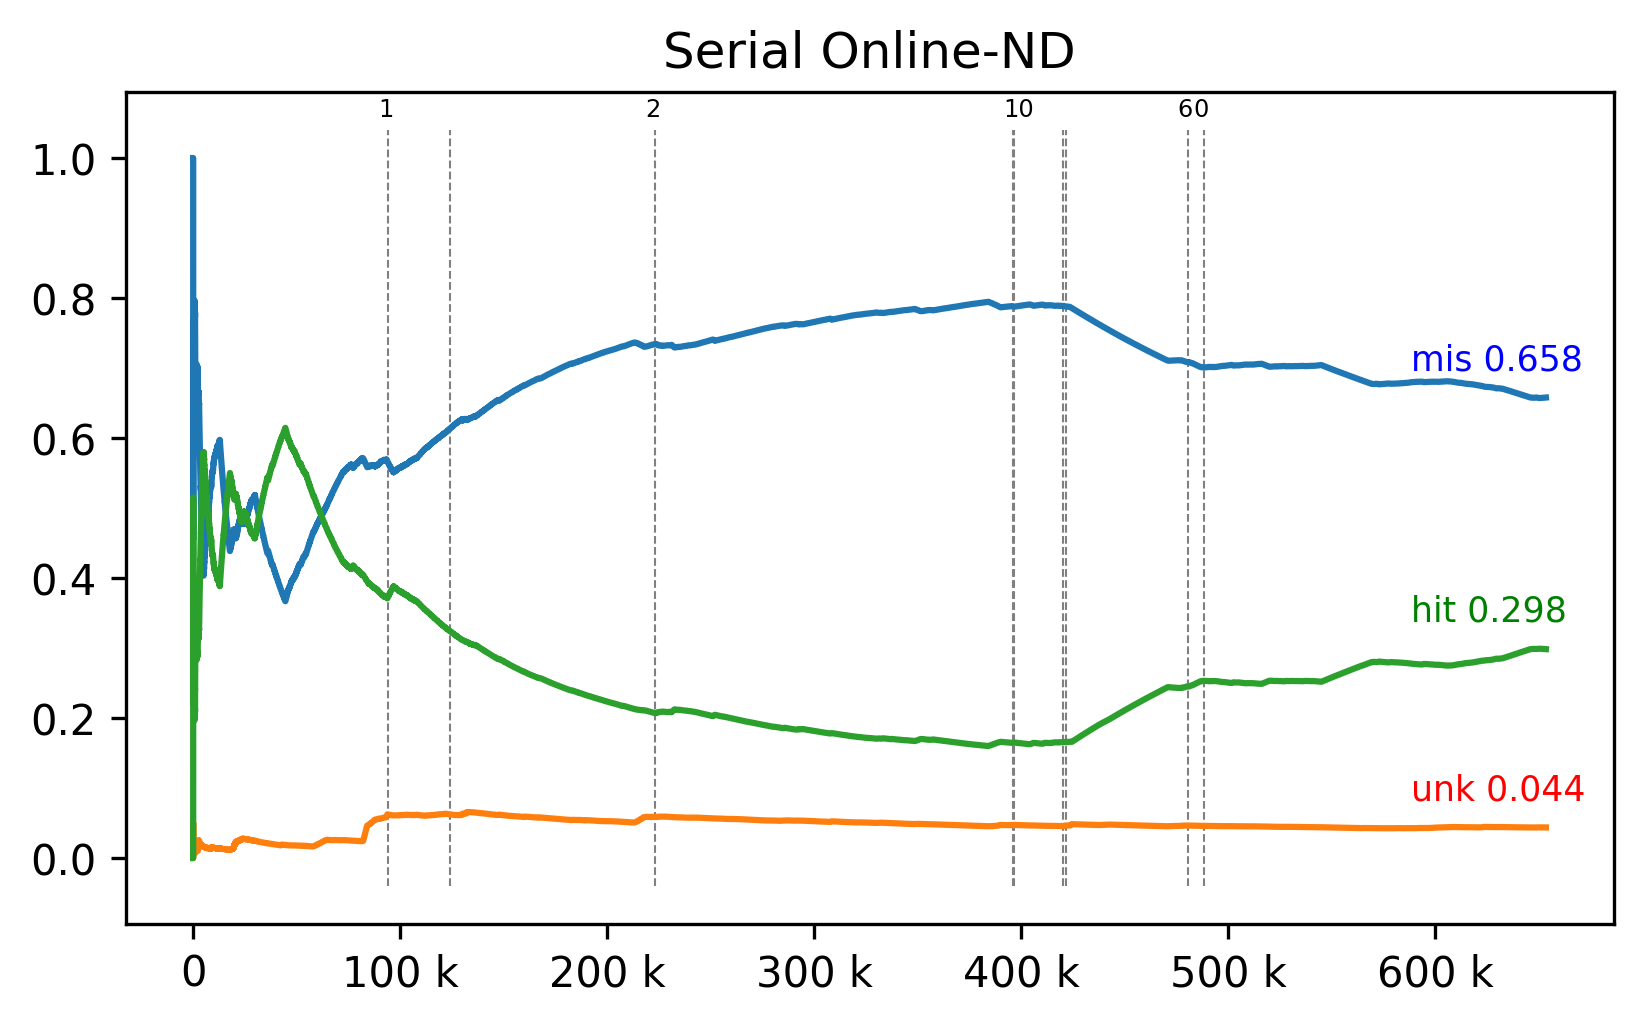
\includegraphics[width=\linewidth]{experiments/online-nd.log.png}
      \caption{Serial Implementation}
      \label{fig:validation-sub-serial}
    \end{subfigure}
  }
  \caption{Validation Comparison: Stream hits and novelties visualization}
  \label{fig:validation-java-serial}
\end{figure*}

% \hl{END Oritações de leitura das métricas e visualizações.}

\subsection{Results Discussion}

Four main experiments need detailed discussion:
(\emph{a}) reference implementation of Minas (\refminas) \cite{Faria2016minas};
(\emph{b}) new implementation in serial mode;
(\emph{c}) new implementation in single-node, multi-task mode and
(\emph{d}) new implementation in multi-node, multi-task mode.
Each experiment uses the adequate binary executable, initial model
(or training set for the reference implementation) and test set
to compute a resulting output stream which is stored for qualitative evaluation.
The summary of all four experiments is shown in Table \ref{tab:exper-summary}.

\begin{table}[hbt]\begin{center}
  \caption{Collected Metrics Summary. \color{red}{deixo os tempos com ou sem a soma do tempo offline?}}
  % \begin{tabular}{l|r|r|r|r}
%          &    Exp. (a)  & Exp. (b)   & Exp. (c)    & Exp. (d)   \\\hline
% Hits     &     0.305618 &   0.298438 &    0.312416 &    0.312478    \\\hline
% Misses   &     0.676049 &   0.657843 &    0.664061 &    0.663802    \\\hline
% Unknowns &     0.018333 &   0.043717 &    0.023521 &    0.023718    \\\hline
% Time     &  2761.830000 &  80.790000 &  522.100000 &  207.140000    \\\hline
% System   &     7.150000 &  11.510000 &   47.770000 &  157.610000    \\\hline
% Elapsed  &  2772.070000 &  93.030000 &  145.040000 &   95.380000    
% \end{tabular}

% java -ea -classpath bin/minas/revised.jar: NoveltyDetection.MinasRevised datasets/training.csv datasets/test.csv out/revised-java.log true
% 	2761.82 user	7.15 system	46:12.07 elapsed

% ./bin/offline
% 	193.94 user	0.05 system	3:14.04 elapsed

% "./bin/ond
% 	80.79 user	11.51 system	1:33.02 elapsed

% mpirun -n 12 -hostfile ./conf/hostsfile ./bin/tmpi
% 	207.13 user	157.61 system	1:35.38 elapsed

\newcommand{\mr}[1]{\multirow{2}{*}{#1}}

\begin{tabular}{l|r|r|r|r|r}
                & \refminas (a)  & Offline       & Serial (b)      & Single Node (c) & Multi Node (d)  \\\hline
\mr{Hits}       & $\ 199708\ $   &               & $\ 195017\ $    & $\ 204151\ $    & $\ 204191\ $    \\
                & $\ 0.305618\ $ &               & $\ 0.298438\ $  & $\ 0.312416\ $  & $\ 0.312478\ $  \\
\hline
\mr{Misses}     & $\ 441769\ $   &               & $\ 429873\ $    & $\ 433936\ $    & $\ 433767\ $    \\
                & $\ 0.676049\ $ &               & $\ 0.657843\ $  & $\ 0.664061\ $  & $\ 0.663802\ $  \\
\hline
\mr{Unknowns}   & $\ 11980\ $    &               & $\ 28567\ $     & $\ 15370\ $     & $\ 15499\ $     \\
                & $\ 0.018333\ $ &               & $\ 0.043717\ $  & $\ 0.023521\ $  & $\ 0.023718\ $  \\
\hline
Time            & $\ 2761.83\ $  & $\ 194.12\ $  & $\ 80.79000\ $  & $\ 522.1000\ $  & $\ 207.1400\ $  \\\hline
System          & $\ 7.15\ $     & $\  0.075\ $  & $\ 11.51000\ $  & $\  47.7700\ $  & $\ 157.6100\ $  \\\hline
Elapsed         & $\ 2772.07\ $  & $\ 194.27\ $  & $\ 93.03000\ $  & $\ 145.0400\ $  & $\  95.3800\ $  
\end{tabular}


  \label{tab:exper-summary}
\end{center}\end{table}

The first two experiments (\emph{a} and \emph{b}) comparison does serve as
validation for our implementation, while the latter three (\emph{b}, \emph{c}
and \emph{d}) serves as showcase for the effects of distribution.

As stated, to validate our implementation we compare it to \refminas
(the original \minas companion implementation), so we extracted the same metrics
using same process for both \emph{a} and \emph{b}, they can be viewed on
Tables \ref{tab:java-matrix}, \ref{tab:libc-matrix} and for ease of comparison
on Table \ref{tab:exper-summary} the summary can be compared side by side.

In general the observed classification quality metrics are very similar,
they diverge slightly where \emph{a} has more \emph{Hits} and \emph{Misses}
whereas \emph{b} shifted those to \emph{Unknowns}.
This phenomenon was watched very closely during development and we found that
small changes to MINAS parameters, MINAS internals like K-means ordering,
cluster edge inclusion and cluster radius formula as stated in
Subsection \ref{sec:implementation}.
As for the efficiency metrics on Table \ref{tab:exper-summary}
our implementation used less time to analyze the test data set,
this is due to small optimizations on the minimal sample to cluster center
on the classifier task and more importantly on the stop condition
on the internal K-means algorithm, while \refminas uses a fixed iteration
limit of $100$, our implementations adds the ``no improvment'' check
and thus stops earlier on most cases and this in turn reduces time taken
on the Novelty Detection step.
Also note that \refminas time includes the Offline phase while
our implementation runs it once and reuses the initial model for
\emph{b}, \emph{c} and \emph{d}.

As for the effects of running a MPI cluster with our implementation
we observe an increase of time when e go from 
\st{we have to say it is pretty shitty because of our choice of distribution 
using round-robin, use some load balancing and micro-batching for better results.}
Nevertheless, we can also show the effects of delay in the
Classify, Novelty Detect, Model Update and Classify loop, as in the
first non-serial experiment \emph{b} we observe a reduction in Novelty Labels
on the Confusion Matrix (Tables \ref{tab:libc-matrix} and \ref{tab:single-node-matrix})
from $10$ to $4$.
The same effect is observed on the stream visualization as well, where
Figure \ref{fig:validation-sub-serial}

% \todo{discutir o delay de 80k entre etiqueta 0 em serial vs node}

When observing the stream visualization on figure \ref{fig:cluster-sub-multi}

\begin{table}[htb]
\begin{subtable}[h]{0.9\textwidth}\begin{center}
    \caption{Parallel single-node}
    \begin{tabular}{l|r|r|r|r|r|r|r}

Labels &      - &       N &    0 &    1 &   2 &  3 &  4 \\\hline
Classes  &        &         &      &      &     &    &    \\\hline
\hline
A        &  12282 &  433797 &  147 &  952 &   0 &  0 &  1 \\\hline
N        &   3088 &  203019 &   40 &   99 &  27 &  5 &  0 \\\hline
\hline
Assigned &      - &       N &    A &    A &   N &  N &  A \\\hline
Hits     &      0 &  203019 &  147 &  952 &  27 &  5 &  1 
\end{tabular}
% \begin{tabular}{l|r}

% Metric   &       Value \\\hline
% \hline
% Hits     &    0.312416 \\\hline
% Misses   &    0.664061 \\\hline
% Unknowns &    0.023521 \\\hline
% Time     &  522.100000 \\\hline
% System   &   47.770000 \\\hline
% Elapsed  &  145.040000 
% \end{tabular}

    \label{tab:single-node-matrix}
\end{center}\end{subtable}
\begin{subtable}[h]{0.9\textwidth}\begin{center}
    \caption{Parallel multi-node}
    \begin{tabular}{l|r|r|r|r|r|r|r}

Labels &      - &       N &    0 &    1 &    2 &    3 &  4 \\\hline
Classes  &        &         &      &      &      &      &    \\\hline
\hline
A        &  12378 &  433631 &  117 &  886 &    0 &  162 &  5 \\\hline
N        &   3121 &  202916 &   40 &   96 &  105 &    0 &  0 \\\hline
\hline
Assigned &      - &       N &    A &    A &    N &    A &  A \\\hline
Hits     &      0 &  202916 &  117 &  886 &  105 &  162 &  5 
\end{tabular}
% \begin{tabular}{l|r}

% Metric   &       Value \\\hline
% \hline
% Hits     &    0.312478 \\\hline
% Misses   &    0.663802 \\\hline
% Unknowns &    0.023718 \\\hline
% Time     &  207.140000 \\\hline
% System   &  157.610000 \\\hline
% Elapsed  &   95.380000 
% \end{tabular}

    \label{tab:multi-node-matrix}
\end{center}\end{subtable}
\caption{Confusion Matrix and Qualitative Metrics for MPI Clusters.}
\label{tab:confusion-matrixes}
\end{table}

% 22.40 user	0.02 system	0:22.48 elapsed

% \begin{table*}[htb]\begin{center}
%   \caption{Serial implementation: Confusion Matrix and Qualitative Metrics}
%   \begin{tabular}{l|r|r|r|r|r|r|r|r|r|r|r}

Labels &      - &       N &   0 &    1 &    2 &   4 &   5 &  6 &   7 &   8 &  10 \\\hline
Classes  &        &         &     &      &      &     &     &    &     &     &     \\\hline
\hline
A        &  16086 &  429765 &  94 &  995 &  104 &   0 &  23 &  3 &  29 &  46 &  34 \\\hline
N        &  12481 &  193642 &   3 &   94 &    0 &  47 &   0 &  0 &   0 &  11 &   0 \\\hline
\hline
Assigned &      - &       N &   A &    A &    A &   N &   A &  A &   A &   A &   A \\\hline
Hits     &      0 &  193642 &  94 &  995 &  104 &  47 &  23 &  3 &  29 &  46 &  34 
\end{tabular}
% \begin{tabular}{l|r}

% Metric   &      Value \\\hline
% Metric   &            \\\hline
% \hline
% Hits     &   0.298438 \\\hline
% Misses   &   0.657843 \\\hline
% Unknowns &   0.043717 \\\hline
% Time     &  80.790000 \\\hline
% System   &  11.510000 \\\hline
% Elapsed  &  93.030000 
% \end{tabular}

%   \label{tab:libc-matrix}
% \end{center}\end{table*}

\begin{figure*}[htb]
  \centerline{
    \begin{subfigure}{.5\textwidth}
      \centering
      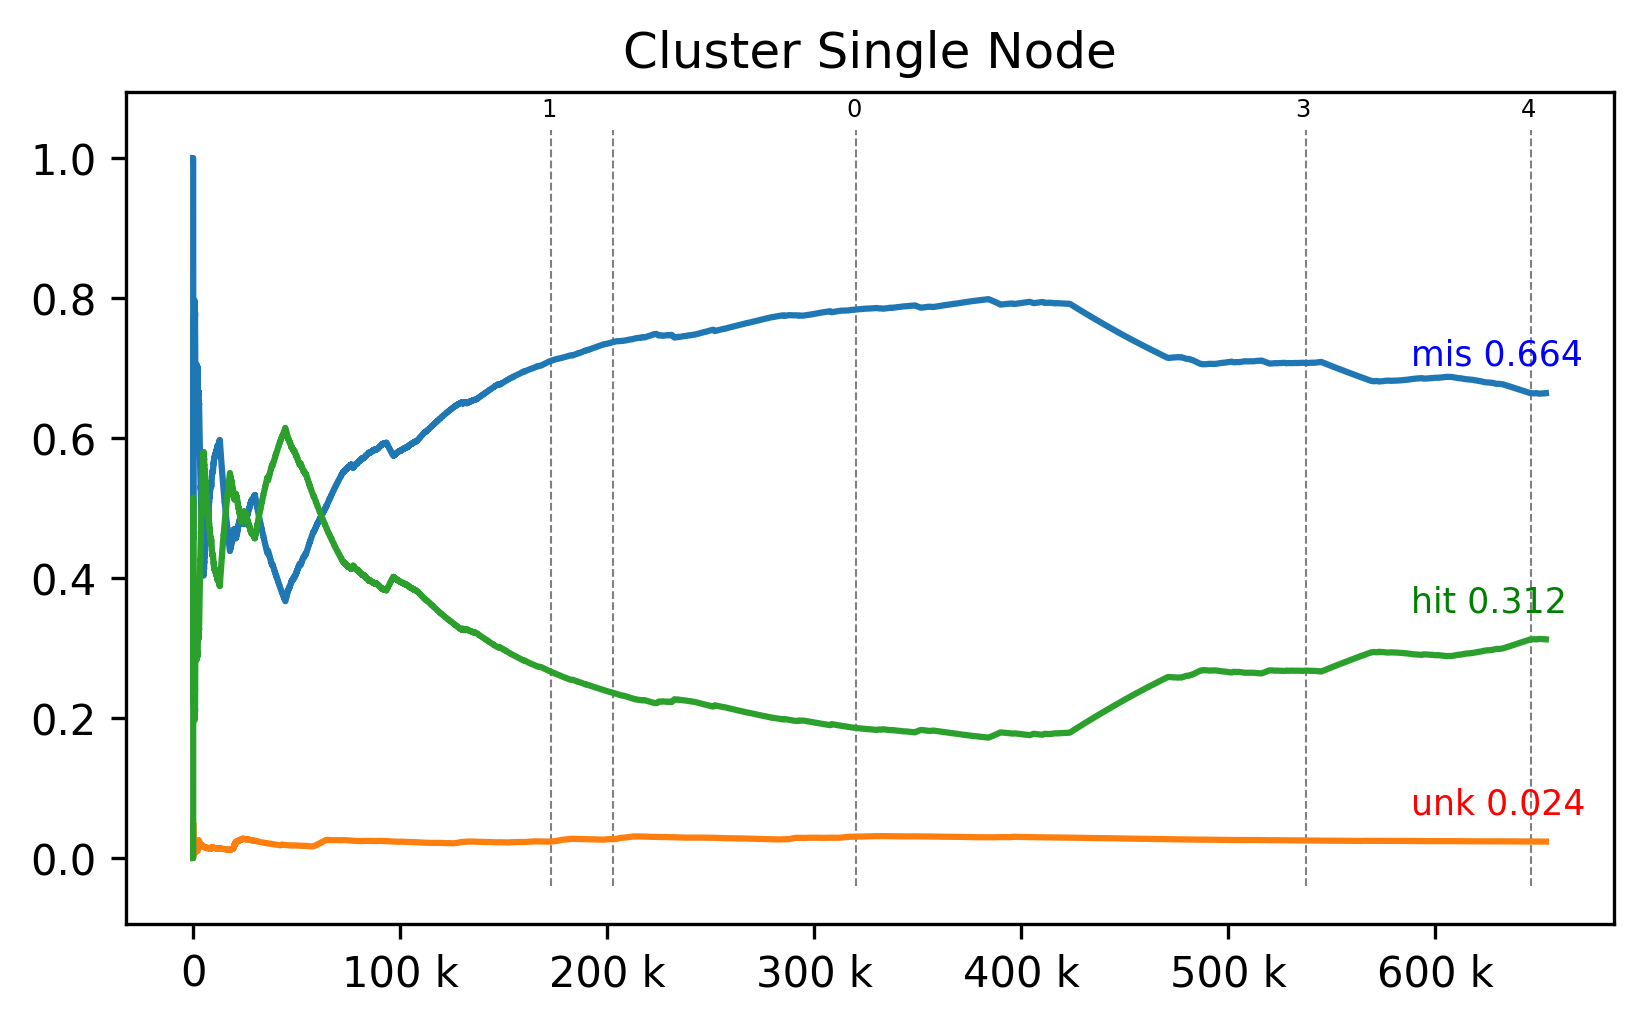
\includegraphics[width=\linewidth]{experiments/tmi-base.log.png}
      \caption{Parallel single-node}
      \label{fig:cluster-sub-single}
    \end{subfigure}
    \begin{subfigure}{.5\textwidth}
      \centering
      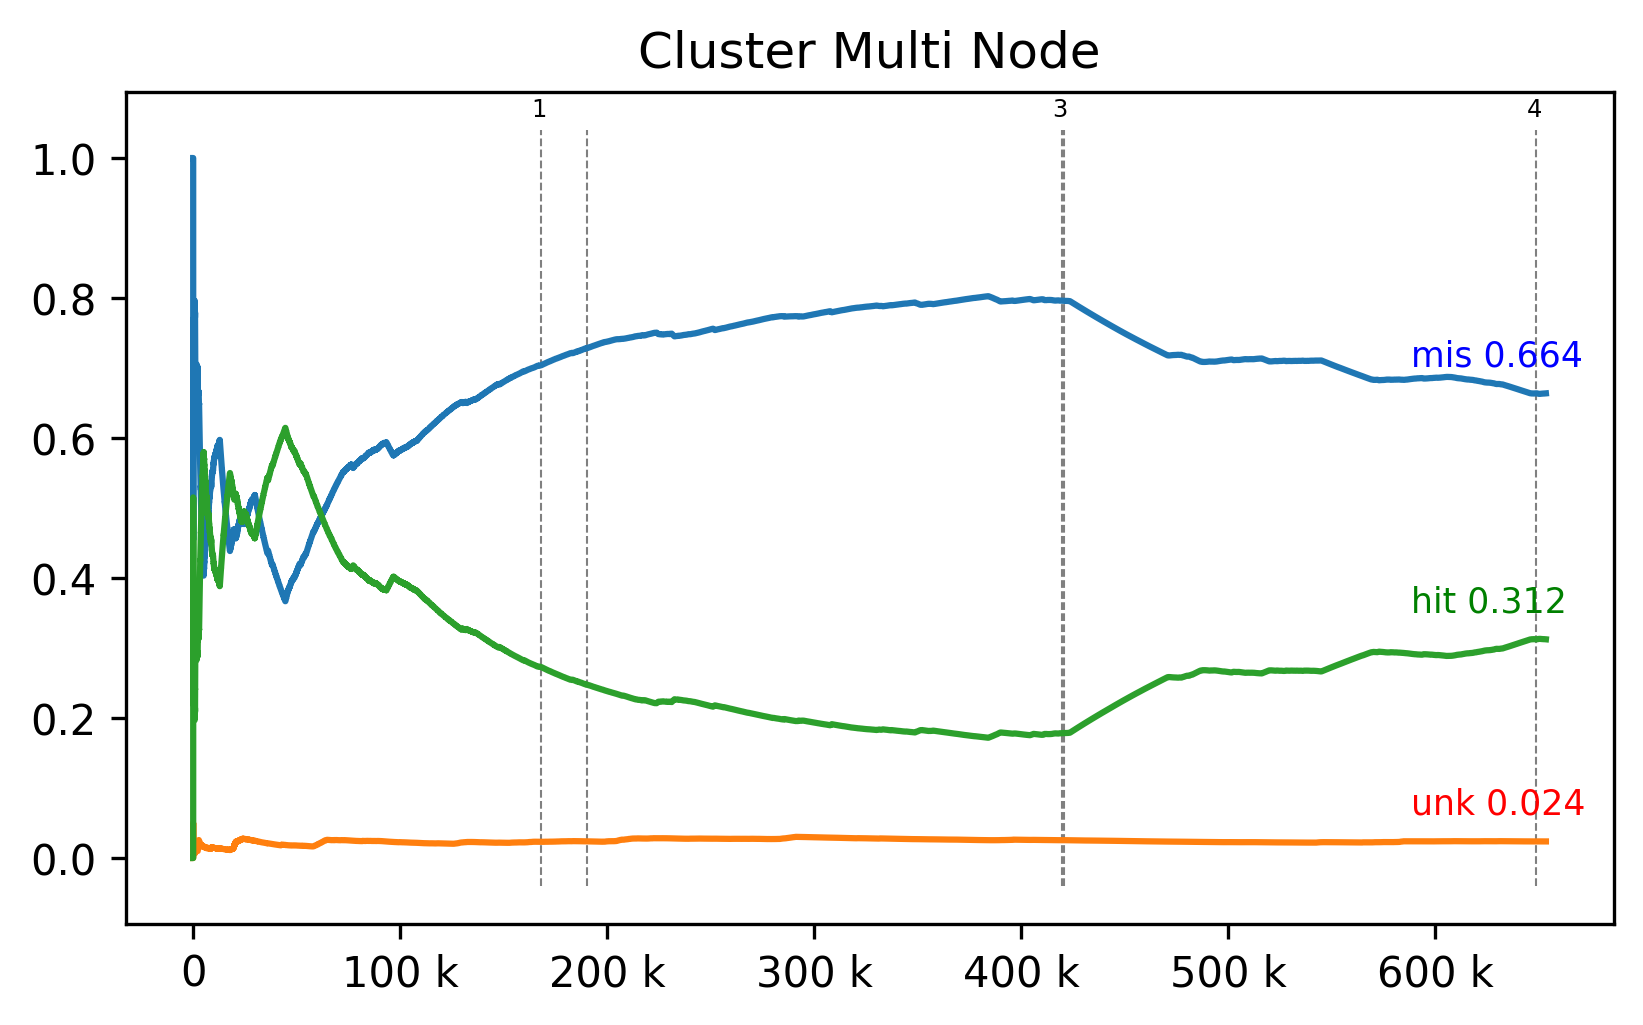
\includegraphics[width=\linewidth]{experiments/tmi-n12.log.png}
      \caption{Parallel multi-node}
      \label{fig:cluster-sub-multi}
    \end{subfigure}
    % \begin{subfigure}{.5\textwidth}
    %   \centering
    %   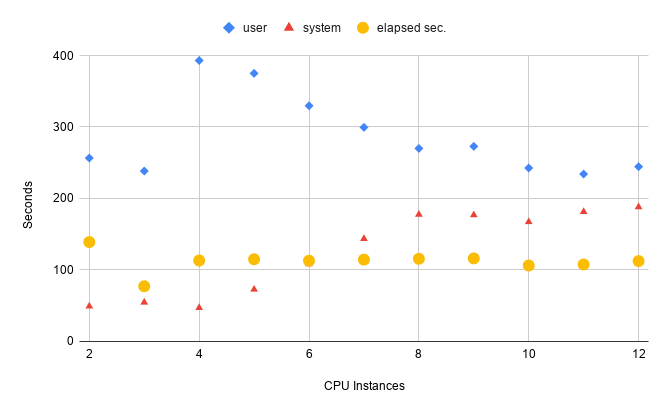
\includegraphics[width=\linewidth]{experiments/speedup-clean.png}
    %   \caption{Time measurements per added instance}
    %   \label{fig:cluster-sub-multi}
    % \end{subfigure}
  }
  \caption{Parallelism Comparison: Stream hits and novelties visualization}
  \label{fig:cluster}
\end{figure*}

\begin{figure}
  \centering
  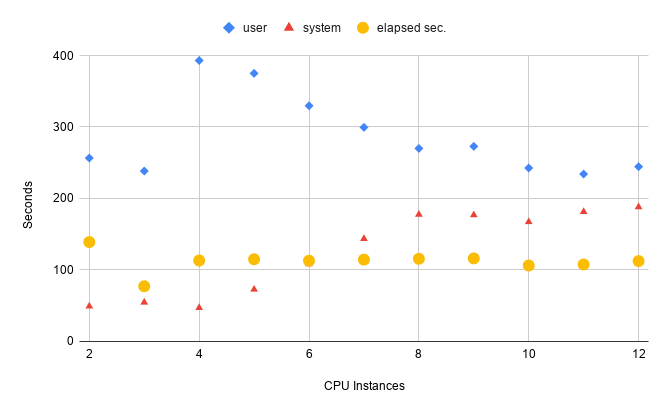
\includegraphics[width=\linewidth]{experiments/speedup-clean.png}
  \caption{Time measurements per added instance}
  \label{fig:speedup}
\end{figure}

% \begin{table}[htb]\begin{center}
%   \caption{Parallel single-node: Confusion Matrix and Qualitative Metrics}
%   \begin{tabular}{l|r|r|r|r|r|r|r}

Labels &      - &       N &    0 &    1 &   2 &  3 &  4 \\\hline
Classes  &        &         &      &      &     &    &    \\\hline
\hline
A        &  12282 &  433797 &  147 &  952 &   0 &  0 &  1 \\\hline
N        &   3088 &  203019 &   40 &   99 &  27 &  5 &  0 \\\hline
\hline
Assigned &      - &       N &    A &    A &   N &  N &  A \\\hline
Hits     &      0 &  203019 &  147 &  952 &  27 &  5 &  1 
\end{tabular}
% \begin{tabular}{l|r}

% Metric   &       Value \\\hline
% \hline
% Hits     &    0.312416 \\\hline
% Misses   &    0.664061 \\\hline
% Unknowns &    0.023521 \\\hline
% Time     &  522.100000 \\\hline
% System   &   47.770000 \\\hline
% Elapsed  &  145.040000 
% \end{tabular}

%   \label{tab:single-node-matrix}
% \end{center}\end{table}

% \setcounter{MaxMatrixCols}{20}
% \begin{table*}[htb]
  %   \begin{center}
    %     \caption{Reference implementation: Confusion Matrix and Qualitative Metrics}
    %     \begin{math}\begin{pmatrix}
      %       - & N & 1 & 2 & 3 & 4 & 5 & 6 & 7 & 8 & 9 & 10 & 11 & 12
%     \end{pmatrix}\end{math}
%     \begin{math}\begin{pmatrix}
%     3774 &  438750 &  123 &  145 &  368 &  8 &  52 &  165 &    1 &  1046 &  161 &  2489 &   71 &  26 \\
%     8206 &  193030 &    0 &   79 &   44 &  0 &   0 &    0 &  229 &   181 &  154 &  4066 &  289 &   0
%     \end{pmatrix}\end{math}
%     \begin{math}\begin{pmatrix}
%       - &       N &    A &    A &    A &  A &   A &    A &    N &     A &    A &     N &    N &   A \\
%       0 &  193030 &  123 &  145 &  368 &  8 &  52 &  165 &  229 &  1046 &  161 &  4066 &  289 &  26 
%     \end{pmatrix}\end{math}
%     \label{math-tab}
%   \end{center}
% \end{table*}

% \begin{figure*}
%   \centering
%   \centerline{
%     \includegraphics[width=0.45\textwidth]{../experiments/revised-java.log.png}
%     \includegraphics[width=0.45\textwidth]{../experiments/revised-java.log.png}
%   }
%   \\
%   \centerline{
%     \includegraphics[width=0.45\textwidth]{../experiments/revised-java.log.png}
%     \includegraphics[width=0.45\textwidth]{../experiments/revised-java.log.png}
%   }
% \label{fig1} 
% \end{figure*}

% \begin{highlight}

% \end{highlight}

